\subsection*{Our investigation}

In order to test how well the spherical k-means clustering algorithm
worked, we constructed a random data set using the Von Mises distribution
random sampling function from the MATLAB Circular Statistics Toolbox\cite{circstats}.
We constructed 70 clusters of 10 points each, using random points
on the sphere as means and with $\kappa=100$, and then applied the
spherical k-means clustering and visualized the results on the unit
three dimensional sphere, color coded for each cluster and with estimated
means labeled as red $X$'s and true means labeled as black $X$'s.

\begin{figure}


\caption{Plot of 70 clusters and means on a 3-D sphere}


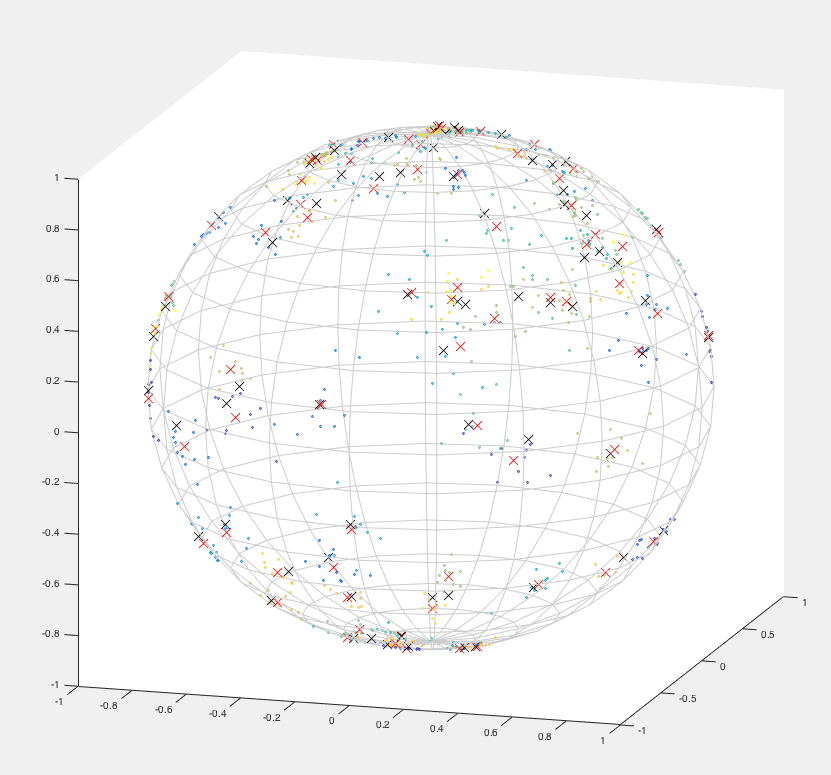
\includegraphics[width=1\textwidth]{sphere_points_70_clusters}
\end{figure}


\begin{figure}
\caption{Plot of 10 clusters and means on a 3-D sphere}


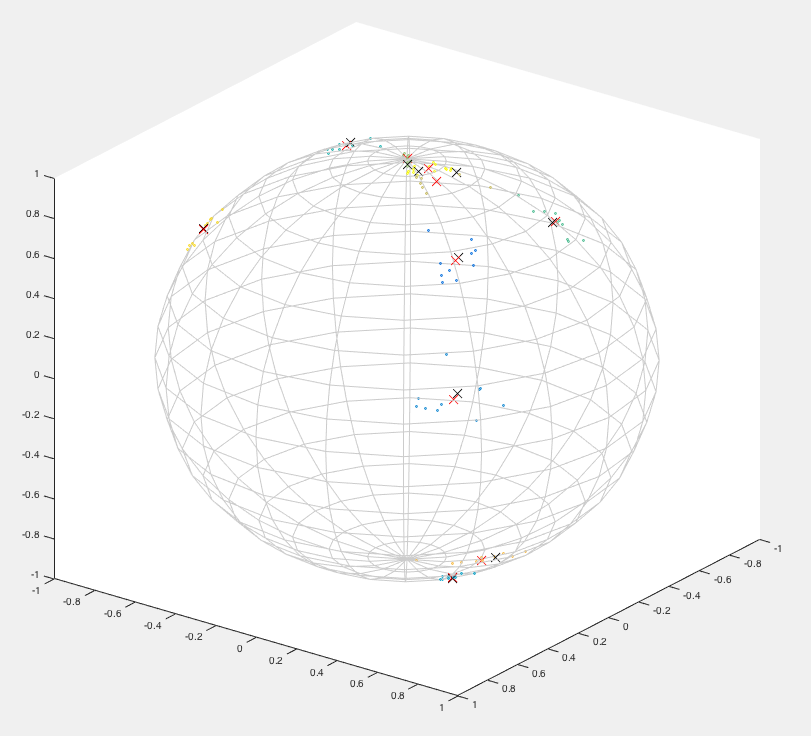
\includegraphics[width=1\textwidth]{sphere_points_10_clusters}
\end{figure}
